\section{Meilenstein 3: 22.05.2019 - 03.07.2019}
Der dritte Meilenstein hatte in erster Linie das formulierte Ziel, dass ein Nutzer sich anhand eines selbst gewählten Start- und Endpunktes und unter Berücksichtigung von real gemessenen und simulierten Feinstaubdaten routen lassen kann.
Um dieses Ziel zu erreichen, müssen zudem die offenen Anforderungen aus Meilenstein 2 umgesetzt werden, sodass der vollständige technische Durchstich erreicht wird.
Durch die Sensorknoten sollen Daten gemessen werden, welche in der IoT"=Plattform gespeichert und bereitgestellt werden.
Diese Daten fließen dann in die Berechnung einer Route ein, die anhand eines Start- und Enpunktes vom Navigationsnutzer vorgegeben wird.


Neben dem formulierten Ziel aus Meilenstein 3, werden auch die ersten Anforderungen zum UIS"=Nutzer umgesetzt.
Für die Umsetzung dieser Anforderungen wird zunächst ein neues Projekt aufgesetzt, welches ein eigenes Frontend als Single Page Webseite beinhaltet.
In diesem soll es interessierten Personen ermöglicht werden, die Sensorknoten"=Abdeckung in Oldenburg in einer Karte einzusehen sowie die gemessenen Feinstaubdaten  zu den jeweiligen Sensorknoten.
Um die Daten im Frontend anzeigen zu können, müssen diese zunächst von der IoT"=Plattform abgefragt werden.
Hierfür können zum Teil bereits bestehende Schnittstellen genutzt werden.


Weiterhin ist im Hauptziel des Meilensteins die Rede von simulierten Werten.
In diesem Zusammenhang soll es die Möglichkeit geben, virtuelle Sensorknoten anzulegen und mit den gleichen Informationen (Standort, Id, Höhe...) zu versehen.
Diese Werte sollen dann im Routing"=Service genauso berücksichtigt werden, wie die real gemessenen Daten.
So wird beispielsweise die Möglichkeit geboten, die Abdeckung von Oldenburg mit Feinstaubdaten zu erhöhen.
Dabei muss jedoch berücksichtigt werden, dass im dritten Meilenstein nur eine Strategie umgesetzt wird, in der in einem bestimmten Intervall festgelegte Werte von den virtuellen Sensorknoten gesendet werden.
Im weiteren Verlauf der Projektgruppe sollen weitere Strategien hinzukommen, in denen zum Beispiel die realen Sensorknoten berücksichtigt werden, sodass durch räumliche Interpolation oder andere Verfahren realistische Werte für die virtuellen Sensorknoten erzeugt werden.

\begin{figure}[!htb]
	\centering
	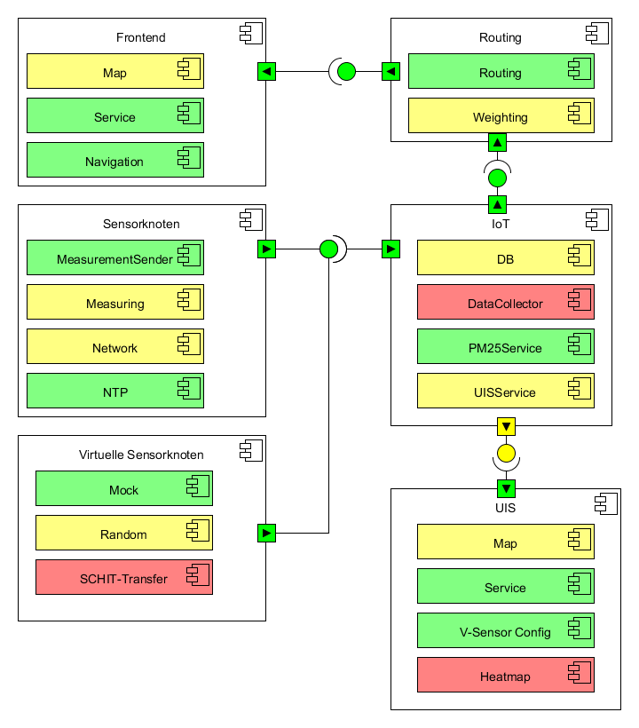
\includegraphics[width=\textwidth]{./ressourcen/bigpicture2.png}
	\caption{Big Picture des dritten Meilensteins}
	\label{fig:bigpicture2}
\end{figure}


Zusammenfassend zeigt sich, dass wieder ein hoher Aufwand an Abstimmungen und Integration zwischen den einzelnen Projekten notwendig ist.
Als Ergebnis des Meilensteins lässt sich festhalten, dass die Schnittstellen zwischen allen System funktionsfähig sind und hier nahezu alle Ziele erreicht worden sind.
Dies zeigt sich auch in \Fig{bigpicture2}.
Jedoch sind auch noch wenige Aufgaben offen, wie das Persistieren von Daten in der Datenbank oder die Integration der Schit"=Daten.
Die in diesem Zusammenhang ausgebrachten Sensorknoten senden momentan noch an eine extra dafür aufgesetzte Plattform.
Um die Daten der Sensorknoten an unser neues System senden zu lassen, sodass die Sensorknoten im Routing berücksichtigt und im UIS"=Frontend angezeigt werden können, muss die Firmware entsprechend geupdated werden.
Aus Zeitgründen und in Hinblick auf die hauptsächlichen Ziele des Meilensteins, wurde die Umsetzung dieser Aufgaben niedriger priorisiert.
Aus diesem Grund wurde eine solche Anforderung im dritten Meilenstein nicht mehr realisiert.
Im Meilenstein ist neben der Umsetzung der offen gebliebenen Anforderungen aus Meilenstein 3 die Möglichkeit des Routens anhand von Temperaturdaten oder anderen vorgesehen.
Dafür muss unter anderem die Sensorknoten"=Firmware erweitert werden, sodass der BME280 die Temperatur, Luftdruck und Luftfeuchte misst, die Werte an die IoT"=Plattform sendet, welche die Werte dann für weitere Services, wie den Routing"=Service bereitstellt.